\documentclass[11pt,a4paper]{article}
\usepackage[utf8]{inputenc}
\usepackage[T1]{fontenc}
\usepackage[brazil]{babel}
\usepackage[margin=2.4cm]{geometry}
\usepackage{booktabs}
\usepackage{amsmath,amssymb}
\usepackage{caption}
\usepackage{graphicx}
\usepackage{setspace}
\usepackage{xcolor}
\usepackage{mdframed}
\usepackage{enumitem}
\usepackage[hidelinks]{hyperref}
\graphicspath{{docs/}}

\onehalfspacing
\captionsetup{font=small,labelsep=colon}

\definecolor{feitog}{RGB}{0,120,60}
\definecolor{fazerb}{RGB}{180,90,0}
\newcommand{\feito}{\textcolor{feitog}{\textbf{[FEITO]}}}
\newcommand{\fazer}{\textcolor{fazerb}{\textbf{[A FAZER]}}}
\newcommand{\futuro}{\textcolor{fazerb}{\textbf{[FUTURO]}}}

\newmdenv[linewidth=0.6pt,linecolor=gray,backgroundcolor=gray!6,
  innertopmargin=6pt,innerbottommargin=6pt,skipabove=8pt,skipbelow=8pt]{conceito}

\title{\textbf{Guia consolidado do projeto}\\[4pt]
\large Demanda institucional por ativos: o peso de VALE3 nas carteiras dos fundos do Itaú\\[6pt]
\normalsize Documento de trabalho --- o que já foi feito, o que falta fazer,\\
com conceitos, equações, resultados e interpretações}
\author{João Paulo Zangrandi \quad (orientador: Prof.\ Maurício Ferraresi Jr.)}
\date{\today}

\begin{document}
\maketitle

\begin{conceito}
\noindent\textbf{Como ler este documento.} Este não é a monografia que vai para a banca; é
um \emph{guia de estudo} para retomar o fio do projeto. Cada parte explica o conceito em
linguagem simples, mostra a equação e interpreta o resultado. As etapas estão marcadas com
\feito{} (já implementado e rodado em R), \fazer{} (próximo passo combinado) ou \futuro{}
(planejado para mais adiante). Os números vêm dos scripts do repositório
\texttt{forecasting-fund-weights-vale-itau}.
\end{conceito}

\tableofcontents
\bigskip

% ======================================================================
\section{O mapa do projeto em uma página}

\paragraph{A pergunta.} Quando um fundo de investimento monta a carteira, ele decide
\emph{quanto} de cada ação vai carregar. Esse ``quanto'', medido como \textbf{peso}
(a fração da carteira na ação, um número entre 0 e 1), é uma medida de \textbf{demanda}.
A pergunta do projeto é dupla:
\begin{enumerate}[topsep=2pt,itemsep=1pt]
\item \textbf{Explicação:} quais \emph{características} de um fundo (tamanho, número de
cotistas, tipo de fundo, fluxo de dinheiro) explicam o peso que ele dá a uma ação?
\item \textbf{Previsão:} esse peso pode ser \emph{previsto} de um mês para o outro?
\end{enumerate}

\paragraph{O caso concreto.} Para tornar o problema tratável, fixamos uma ação, \textbf{VALE3}
(posição direta), e uma gestora, o grupo \textbf{Itaú} (Asset, DTVM e Unibanco), no período
\textbf{2016--2021} (72 meses). Estuda-se como o peso de VALE3 varia entre os fundos do Itaú e
ao longo do tempo.

\paragraph{A estratégia (em dois passos).} (i) A cada mês, regredimos o peso da ação nas
características dos fundos; os coeficientes dessa regressão resumem ``como as posições dependem
das características'' --- são um \textbf{fator latente} $\theta_t$. (ii) Deixamos esse fator
\emph{variar no tempo} e tentamos prever o peso, comparando com a \textbf{previsão ingênua}
(repetir o último peso).

\paragraph{O que já sabemos.} As características \emph{explicam bem} o peso (sinais estáveis nos
72 meses), mas \emph{não conseguem prevê-lo} melhor do que simplesmente repetir o último valor:
no nível do fundo, o peso é quase um \textbf{passeio aleatório}. Esse contraste é o eixo do
trabalho.

\paragraph{Para onde vamos.} A agenda combinada com o orientador refina a parte de modelagem em
quatro frentes: padronização e \textbf{erros-padrão Newey-West} (passo 1, já feito); forma
funcional \textbf{logística} para o peso (passo 2); o \textbf{modelo de ajuste parcial} com
estimação por \textbf{variável instrumental} (passo 3); e, mais à frente, \textbf{regularização
(ridge)} para a estimação dos fatores em alta dimensão (passo futuro).

% ======================================================================
\section{Conceitos-chave, em linguagem simples}

\begin{conceito}
\textbf{Sistema de demanda (Koijen e Yogo, 2019).} É a ideia de tratar os preços dos ativos como
o resultado das \emph{demandas} de muitos investidores, e cada demanda é uma função das
\emph{características} dos ativos. A vantagem é trocar um problema gigante (milhares de ativos e
investidores) por um número pequeno de parâmetros ligados a características. \emph{Como nos
afastamos disso:} aqui o ativo é \textbf{fixo} (VALE3) e quem varia são as características do
\emph{fundo}; estimamos a forma reduzida ``pelas quantidades'' (o peso), sem modelar o canal
preço-demanda.
\end{conceito}

\begin{conceito}
\textbf{Características do fundo e fatores latentes da ação.} Chamamos de $x_i$ o vetor de
características do fundo $i$ (tamanho, cotistas etc.) --- o ``perfil'' do fundo. Chamamos de
$\theta_n$ o vetor de \emph{fatores latentes} da ação $n$ --- o quanto cada característica
``puxa'' a posição naquela ação. O peso desejado é, então, o produto $x_i'\theta_n$: o perfil do
fundo vezes a sensibilidade da ação a cada traço do perfil.
\end{conceito}

\begin{conceito}
\textbf{Seção transversal (cross-section) e Fama-MacBeth (1973).} ``Seção transversal'' é uma
fotografia de um mês: todos os fundos ao mesmo tempo. Rodamos uma regressão por mês $\to$ 72
conjuntos de coeficientes. Fama-MacBeth é a receita de resumir essas 72 fotos: tira-se a
\emph{média} de cada coeficiente no tempo e mede-se a incerteza pela \emph{variação} dele entre
os meses.
\end{conceito}

\begin{conceito}
\textbf{Autocorrelação e erros-padrão Newey-West.} Os 72 coeficientes mensais não são
independentes: o de um mês se parece com o do mês anterior (autocorrelação de $\approx0{,}7$ a
$0{,}8$). O erro-padrão clássico de Fama-MacBeth \emph{supõe independência} e, por isso,
\emph{subestima} a incerteza e \emph{infla} as estatísticas $t$. O estimador de \textbf{Newey-West}
corrige isso somando as autocovariâncias (com pesos decrescentes) --- dá erros-padrão maiores e
$t$ menores, porém honestos.
\end{conceito}

\begin{conceito}
\textbf{Resposta fracionária / ligação logística.} O peso vive em $[0,1]$. Uma regressão linear
pode prever valores negativos ou acima de 1, o que não faz sentido. A \emph{função logística}
$g(z)=1/(1+e^{-z})$ espreme qualquer número para dentro de $(0,1)$, respeitando o limite. É a
forma funcional correta para uma fração (Papke e Wooldridge, 1996).
\end{conceito}

\begin{conceito}
\textbf{Ajuste parcial.} A ideia de que o fundo não pula de uma vez para o peso desejado, mas se
move só \emph{parte} do caminho a cada mês, a uma velocidade $\lambda$. Se $\lambda=1$, ajusta
tudo na hora; se $\lambda=0$, não ajusta nada (o peso fica ``preso'' no valor de ontem --- que é
justamente a previsão ingênua).
\end{conceito}

\begin{conceito}
\textbf{Viés de atenuação e variável instrumental.} Quando um regressor é \emph{medido com erro}
(no nosso caso, a ``distância ao alvo'' é construída a partir de coeficientes \emph{estimados}),
o mínimos quadrados puxa o coeficiente \emph{para zero} --- isso é o \textbf{viés de atenuação}.
Como o teste central é justamente ``$\lambda$ é diferente de zero?'', um método que empurra para
zero atrapalha. A \textbf{variável instrumental} (ou correção de erros nas variáveis) conserta
isso usando uma fonte de variação ``limpa'' do regressor.
\end{conceito}

\begin{conceito}
\textbf{Por que ridge agora não, mas no futuro sim.} A \emph{regularização ridge} encolhe
coeficientes em direção a zero para estabilizá-los. Isso é \emph{ruim} para estimar $\lambda$
(agravaria a atenuação contra a hipótese de interesse), mas é \emph{bom} para o primeiro passo
quando o número de características crescer ou quando escalarmos para muitas ações: ali os
regressores são \emph{observados} (sem erro de medida) e o objetivo é estabilizar, não testar se
algo é zero. Por isso o ridge é um \textbf{passo futuro}, não descartado.
\end{conceito}

% ======================================================================
\section{Os dados \feito}

Duas bases da Comissão de Valores Mobiliários e uma fonte de mercado:
\begin{itemize}[topsep=2pt,itemsep=1pt]
\item \textbf{Composição consolidada} (mensal): o peso de VALE3 (posição direta) em cada fundo.
\item \textbf{Série histórica} (diária): patrimônio líquido, número de cotistas, e se o fundo é
um \textbf{fundo de cotas} (FIC, que investe em outros fundos em vez de ações diretamente).
\item \textbf{Informe Diário} (diário): captação e resgate $\to$ \textbf{fluxo líquido}.
\item \textbf{Mercado}: preço e \textbf{beta} de VALE3 (beta = sensibilidade da ação ao
Ibovespa, em janela de 252 pregões).
\end{itemize}

\paragraph{Tratamentos.} Padronização do nome da gestora; remoção de linhas duplicadas e de pesos
negativos (resíduos contábeis); exclusão de fundos exclusivos (mantendo só $>3$ cotistas); junção
das bases pelo dia exato da competência. A captação foi validada contra a série histórica
($>99\%$ de coincidência ao centavo) e o preço contra o fechamento oficial da bolsa.

\paragraph{Amostra.} 72 meses (2016--2021), grupo Itaú. Painel completo de quem detém a ação:
26.123 observações de fundo-mês, 623 fundos. Amostra de regressão (com $>3$ cotistas e fluxo):
\textbf{11.413 observações, 307 fundos}, das quais $\approx76\%$ são fundos de cotas.

\begin{table}[h]\centering\small
\caption{Estatísticas descritivas da amostra de regressão.}
\begin{tabular}{@{}lrrrrr@{}}
\toprule
Variável & Média & Desvio-padrão & Mediana & Mínimo & Máximo \\
\midrule
Peso de VALE3 (\%)            & $2{,}87$ & $3{,}52$ & $1{,}22$ & $0{,}00$ & $23{,}55$ \\
Patrimônio líquido (R\$ mi)   & $399$    & $1.079$  & $68{,}3$ & $0{,}04$ & $17.866$ \\
Número de cotistas            & $10.202$ & $72.039$ & $105$    & $4$      & $696.013$ \\
Captação líquida (R\$ mi)     & $5{,}7$  & $74{,}1$ & $0{,}0$  & $-1.522$ & $1.636$ \\
Preço de VALE3 (R\$)          & $54{,}6$ & $27{,}2$ & $50{,}9$ & $9{,}94$ & $114{,}1$ \\
Beta de VALE3                 & $1{,}04$ & $0{,}30$ & $0{,}97$ & $0{,}68$ & $1{,}73$ \\
\bottomrule
\end{tabular}
\end{table}

\noindent Patrimônio e cotistas são muito assimétricos (média $\gg$ mediana) $\Rightarrow$ usamos
o logaritmo. Preço e beta têm correlação de $\approx-0{,}71$ (na alta de 2016--2021 o preço subiu
e o beta caiu), o que dificulta separar os dois efeitos mais adiante.

% ======================================================================
\section{A metodologia, com todas as equações}

\subsection{Especificação de demanda}
O peso observado é um peso desejado mais um erro. Como o peso é uma fração, o peso desejado passa
por uma ligação logística:
\begin{equation}
w_{i,t} = g\!\left(x_{i,t}'\,\theta_{n,t}\right) + \varepsilon^{w}_{i,t},
\qquad g(z)=\frac{1}{1+e^{-z}},
\label{eq:logit}
\end{equation}
em que $x_{i,t}$ são as características do fundo e $\theta_{n,t}$ os fatores latentes da ação.
A versão \emph{linear} ($g(z)\approx z$) é usada como aproximação no passo transversal; a
logística plena entra na decisão de posse e no modelo de ajuste parcial.

\subsection{Primeiro passo: a regressão transversal (o fator latente)}
Em cada mês $t$, com os fundos empilhados, estimamos por mínimos quadrados
\begin{equation}
\widehat{\theta}_{n,t} = (X_t'X_t)^{-1}X_t'\,w_t,
\label{eq:ols}
\end{equation}
ou seja, mês a mês rodamos
\begin{equation}
w_{i,t} = \alpha_t + \beta^{1}_t\,z(\ln\text{PL})_{i,t} + \beta^{2}_t\,z(\ln\text{Cot})_{i,t}
        + \beta^{3}_t\,\text{FIC}_i + \beta^{4}_t\Big(\tfrac{\text{Fluxo}}{\text{PL}}\Big)_{i,t}
        + \varepsilon_{i,t}.
\label{eq:cs}
\end{equation}
As características de escala $\ln\text{PL}$ e $\ln\text{Cot}$ entram \textbf{padronizadas}
($z(\cdot)$: centradas e divididas pelo desvio-padrão), de modo que o coeficiente é o efeito de
\emph{um desvio-padrão}; FIC fica em 0/1 e o intercepto recupera o nível médio do peso. O resumo
Fama-MacBeth toma a média no tempo,
\begin{equation}
\bar{\beta}_k = \frac{1}{T}\sum_{t=1}^{T}\beta_{k,t}, \qquad T=72.
\label{eq:fm}
\end{equation}

\subsection{Erros-padrão corrigidos (Newey-West) \feito}
Como os $\beta_{k,t}$ são autocorrelacionados, a variância da média é estimada por
\begin{equation}
\widehat{\mathrm{Var}}_{\text{NW}}(\bar{\beta}_k) = \frac{1}{T^{2}}\!\left[
\sum_{t=1}^{T}\widehat{u}_{k,t}^{2}
+ 2\sum_{\ell=1}^{L}\!\left(1-\frac{\ell}{L+1}\right)\!\sum_{t=\ell+1}^{T}\widehat{u}_{k,t}\,\widehat{u}_{k,t-\ell}
\right], \quad \widehat{u}_{k,t}=\beta_{k,t}-\bar{\beta}_k,
\label{eq:nw}
\end{equation}
com $L=3$ (regra $L=\lfloor 4\,(T/100)^{2/9}\rfloor$ para $T=72$). Os resultados estão na
Seção~\ref{sec:res1}.

\subsection{Segundo passo: dinâmica do fator e previsão \feito}
Cada coeficiente $\theta_{k,t}$ é tratado como série temporal (passeio aleatório, AR(1) ou filtro
de Kalman). A previsão do peso é $\widehat{w}_{i,t}=g(\widehat{\theta}_t'x_{i,t})$, comparada à
ingênua $\widehat{w}_{i,t}=w_{i,t-1}$. Avaliamos fora da amostra a 1 e a 3 meses (este último por
causa da \textbf{opacidade}: as carteiras só são divulgadas com $\approx$90 dias de atraso).

\subsection{A decisão de ter ou não a ação (margem extensiva) \feito}
Além de ``quanto'' (margem intensiva), estudamos ``ter ou não'' (margem extensiva) com um painel
que inclui os zeros e uma regressão logística da probabilidade de o fundo deter VALE3.

\subsection{Extensão dinâmica: o modelo de ajuste parcial \fazer}
\label{sec:pa}
O fundo move o peso parcialmente em direção ao desejado, à velocidade $\lambda_n\in(0,1)$:
\begin{equation}
w_{i,t+1} = (1-\lambda_n)\,w_{i,t} + \lambda_n\,w^{*}_{i,t} + u_{i,t+1}.
\label{eq:pa1}
\end{equation}
Definindo a distância ao alvo $d_{i,t}\equiv w^{*}_{i,t}-w_{i,t}$, isso vira
\begin{equation}
w_{i,t+1}-w_{i,t} = \lambda_n\,d_{i,t} + u_{i,t+1}.
\label{eq:pa2}
\end{equation}
A estimativa direta por mínimos quadrados, $\widehat{\lambda}^{\text{MQO}}_n=(d_n'd_n)^{-1}d_n'(\Delta w)$,
sofre \textbf{viés de atenuação}, porque $d_{i,t}=g(x_{i,t}'\widehat{\theta}_n)-w_{i,t}$ usa
$\widehat{\theta}_n$ estimado (erro de medida). Por isso $\lambda$ será estimado por
\textbf{variável instrumental / correção de erros nas variáveis}, e \emph{não} por ridge. O erro
de previsão correspondente é
\begin{equation}
\widehat{u}_{n,t+1} = (w_{n,t+1}-w_{n,t}) - \widehat{\lambda}_n\!\left(g(X_t\widehat{\theta}_n)-w_{n,t}\right).
\label{eq:u}
\end{equation}

% ======================================================================
\section{Resultados já obtidos}
\label{sec:res1}

\subsection{Determinantes do peso, agora com Newey-West \feito}
A Tabela~\ref{tab:nw} traz a regressão mês a mês resumida à Fama-MacBeth, com os dois
erros-padrão lado a lado. \textbf{Leitura dos sinais:} fundos maiores carregam \emph{menos} VALE3
em peso; fundos com mais cotistas carregam \emph{mais}; fundos de cotas têm posição direta
\emph{menor}; a captação do mês não explica o nível do peso. Esses sinais se repetem nos 72 meses.

\begin{table}[h]\centering\small
\caption{Cross-section mês a mês (Fama-MacBeth, $T=72$). Erros-padrão clássico vs.\ Newey-West
($L=3$). Coeficientes não-padronizados (por unidade de log).}
\label{tab:nw}
\begin{tabular}{@{}lrrrrr@{}}
\toprule
Variável & Coef.\ médio & EP clássico & $t$ clássico & EP Newey-West & $t$ Newey-West \\
\midrule
Intercepto              & $0{,}08939$  & $0{,}00413$ & $21{,}6$  & $0{,}00718$ & $12{,}5$  \\
$\ln$(patrimônio)       & $-0{,}00376$ & $0{,}00020$ & $-19{,}3$ & $0{,}00034$ & $-11{,}2$ \\
$\ln$(cotistas)         & $0{,}00387$  & $0{,}00020$ & $19{,}8$  & $0{,}00035$ & $10{,}9$  \\
Fundo de cotas          & $-0{,}01697$ & $0{,}00089$ & $-19{,}2$ & $0{,}00151$ & $-11{,}3$ \\
Captação / patrimônio   & $-0{,}00044$ & $0{,}00309$ & $-0{,}14$ & $0{,}00412$ & $-0{,}11$ \\
\bottomrule
\end{tabular}
\caption*{\footnotesize $R^2$ médio por mês $=0{,}152$. A correção de Newey-West amplia os
erros-padrão em $\approx1{,}7$--$1{,}8\times$. Fonte: \texttt{R/24\_fm\_neweywest.R}.}
\end{table}

\paragraph{O que a correção muda (e o que não muda).} O Newey-West \textbf{não altera os sinais
nem a significância qualitativa}: as características de fundo seguem com $p<0{,}001$ e a captação
segue não significativa. O que muda é a \emph{magnitude} das estatísticas: os $t$ caem de
$\approx 19$--$22$ (clássico) para $\approx 11$--$12{,}5$ (Newey-West). \emph{Observação honesta:}
a versão preliminar do texto mencionava $t$ ``em torno de 19 a 22'' após a correção, mas esses
eram os valores \emph{clássicos}; os corrigidos, calculados aqui, são $\approx 11$--$12{,}5$ ---
ainda fortemente significativos.

\paragraph{Magnitudes por desvio-padrão (versão padronizada).} Padronizando $\ln$PL e $\ln$Cot,
o intercepto vira \textbf{0,0396} ($\approx3{,}96\%$), que é o nível médio do peso de um fundo
não-FIC de tamanho médio. Os efeitos por \emph{um} desvio-padrão são:
\begin{center}\small
\begin{tabular}{@{}lrr@{}}
\toprule
Característica & Coef.\ por desvio-padrão & Leitura \\
\midrule
$\ln$(patrimônio) & $-0{,}00681$ & $+1$ d.p.\ de tamanho $\to$ $-0{,}68$ p.p.\ de peso \\
$\ln$(cotistas)   & $+0{,}01087$ & $+1$ d.p.\ de cotistas $\to$ $+1{,}09$ p.p.\ de peso \\
Fundo de cotas    & $-0{,}01697$ & ser FIC $\to$ $-1{,}70$ p.p.\ de peso \\
\bottomrule
\end{tabular}
\end{center}
\emph{Observação honesta:} os ``$-0{,}38$ / $+0{,}39$ p.p.'' citados na versão preliminar eram os
coeficientes em log \emph{cru} lidos como se fossem por desvio-padrão. Os verdadeiros efeitos por
desvio-padrão são maiores, e o de \emph{cotistas} ($+1{,}09$) supera o de \emph{tamanho}
($-0{,}68$) --- não são ``semelhantes''. Isso reforça que dispersão de cotistas é o traço mais
associado a peso direto maior.

\subsection{Forma logística (resposta fracionária) \feito}
Reestimamos a mesma cross-section, agora com a ligação logística da \eqref{eq:logit} (em R,
\texttt{glm} família \texttt{quasibinomial}), mês a mês. A Tabela~\ref{tab:logit} traz os
coeficientes no resumo Fama-MacBeth com Newey-West.

\begin{table}[h]\centering\small
\caption{Cross-section logística (resposta fracionária), Fama-MacBeth + Newey-West. Coeficientes
na escala de \emph{log-odds}; características de escala padronizadas.}
\label{tab:logit}
\begin{tabular}{@{}lrrrr@{}}
\toprule
Variável & Coef.\ (log-odds) & EP Newey-West & $t$ Newey-West & Meses com sinal $+$ \\
\midrule
Intercepto              & $-3{,}380$ & $0{,}150$ & $-22{,}5$ & 0/72 \\
$\ln$(patrimônio) [d.p.]& $-0{,}339$ & $0{,}043$ & $-7{,}9$  & 0/72 \\
$\ln$(cotistas) [d.p.]  & $+0{,}469$ & $0{,}035$ & $13{,}3$  & 72/72 \\
Fundo de cotas          & $-0{,}732$ & $0{,}062$ & $-11{,}7$ & 0/72 \\
Captação / patrimônio   & $+0{,}078$ & $0{,}183$ & $0{,}43$  & 37/72 \\
\bottomrule
\end{tabular}
\caption*{\footnotesize Fonte: \texttt{R/25\_fractional\_logit.R}.}
\end{table}

\noindent Três pontos resumem o passo:
\begin{enumerate}[topsep=2pt,itemsep=1pt]
\item \textbf{Sinais e significância são idênticos ao linear:} patrimônio e FIC negativos,
cotistas positivo, captação não significativa, todos estáveis nos 72 meses.
\item \textbf{As magnitudes coincidem no centro.} O coeficiente de \emph{log-odds} não é
comparável direto ao linear, mas o \textbf{efeito parcial médio} (a derivada média de $g$, em
pontos de peso) é: dá $-0{,}68$ p.p.\ (patrimônio), $+1{,}06$ p.p.\ (cotistas) e $-1{,}60$ p.p.\
(FIC), praticamente iguais aos coeficientes lineares ($-0{,}68$, $+1{,}09$, $-1{,}70$). Ou seja,
\emph{o linear era uma boa aproximação no centro} --- a conclusão econômica não muda.
\item \textbf{O ganho do logit é respeitar o suporte.} O modelo linear gera previsões
\emph{fora} de $[0,1]$ em $287$ de $11.413$ casos ($2{,}51\%$) --- pesos negativos, sem sentido;
o logit, por construção, nunca. O ajuste também melhora de leve (pseudo-$R^2$ $0{,}165$ vs
$0{,}152$). Isso é exatamente o que o orientador antecipou, e é \textbf{pré-requisito do passo 3},
em que o peso desejado $w^{*}=g(x'\theta)$ precisa estar em $[0,1]$.
\end{enumerate}

\subsection{Versão com preço e beta (dados empilhados) \feito}
Empilhando os 72 meses e acrescentando preço e beta (média do mês), os sinais de fundo se mantêm.
Preço entra positivo (parte é \emph{mecânica}: se a ação sobe, sua fração cresce sozinha); beta
entra negativo (aversão a risco), mas com a ressalva da colinearidade preço-beta ($-0{,}71$):
parte do coeficiente do beta pode estar capturando o resíduo mecânico do preço. $R^2=0{,}166$
(quase igual ao $0{,}152$ sem preço/beta $\Rightarrow$ as características de fundo já carregam a
maior parte da informação).

\begin{table}[h]\centering\small
\caption{Regressão com todos os meses empilhados, incluindo preço e beta (11.413 observações).}
\begin{tabular}{@{}lrrrc@{}}
\toprule
Variável & Estimativa & Erro padrão & $t$ & Sig. \\
\midrule
Intercepto              & $0{,}09937$  & $0{,}00406$ & $24{,}5$   & *** \\
$\ln$(patrimônio)       & $-0{,}00354$ & $0{,}00019$ & $-19{,}0$  & *** \\
$\ln$(cotistas)         & $0{,}00388$  & $0{,}00013$ & $30{,}9$   & *** \\
Fundo de cotas          & $-0{,}01682$ & $0{,}00079$ & $-21{,}3$  & *** \\
Captação / patrimônio   & $-0{,}00030$ & $0{,}00034$ & $-0{,}91$  & n.s. \\
Preço de VALE3          & $0{,}000182$ & $0{,}000016$& $11{,}5$   & *** \\
Beta de VALE3           & $-0{,}02141$ & $0{,}00142$ & $-15{,}1$  & *** \\
\bottomrule
\end{tabular}
\end{table}

\subsection{Dinâmica do fator $\theta_t$ \feito}
Os coeficientes são persistentes mas \emph{revertem à média} (autocorrelação $\approx0{,}7$--$0{,}8$;
o teste de raiz unitária rejeita passeio aleatório puro). Logo, vale modelá-los por AR(1)/Kalman.
A Figura~\ref{fig:theta} mostra os cinco coeficientes; note a reconfiguração comum em torno de
2018 em vários painéis.

\begin{figure}[h]\centering
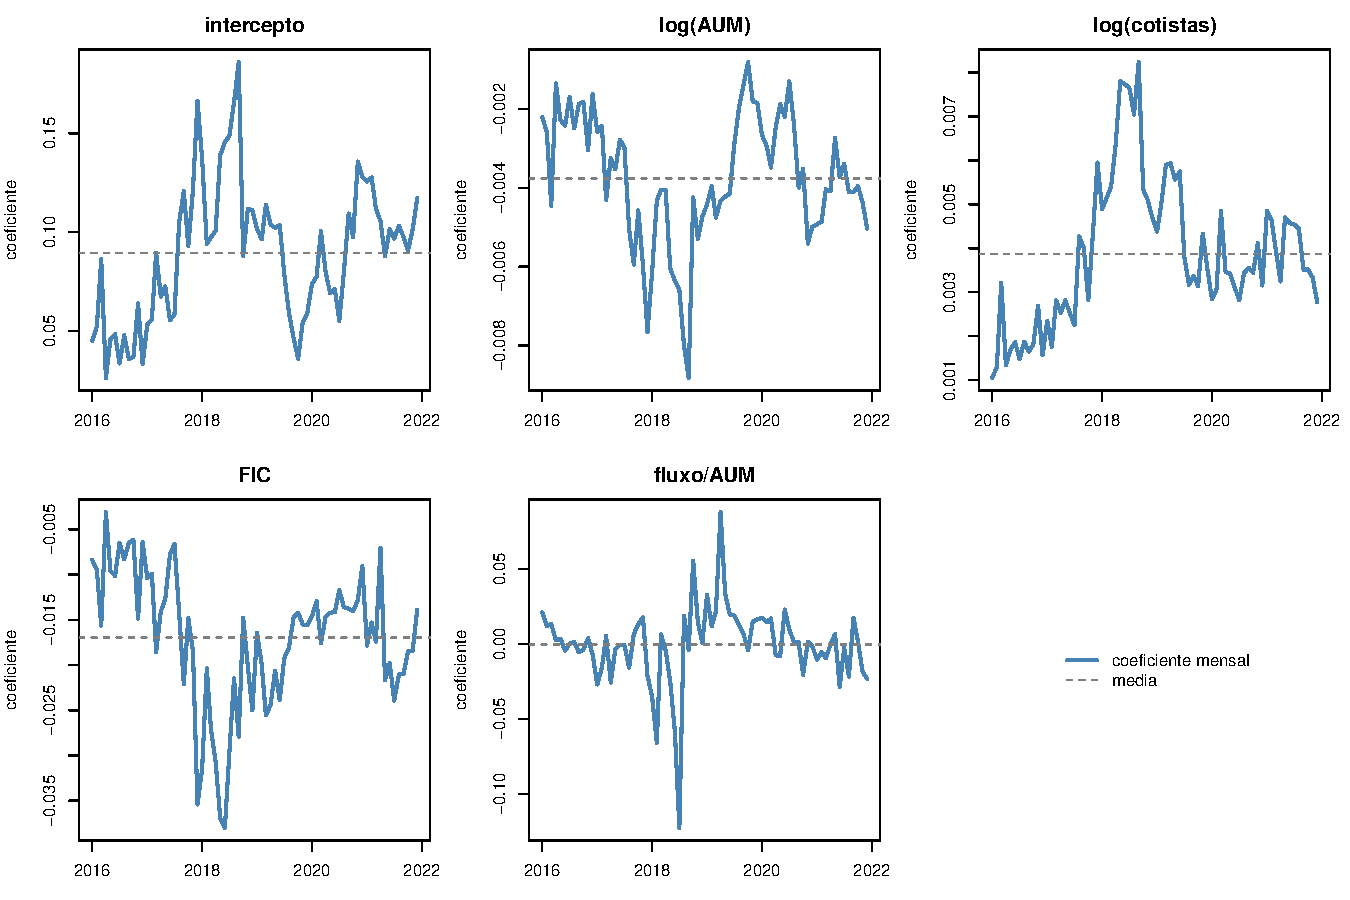
\includegraphics[width=0.80\textwidth]{fig_theta.pdf}
\caption{Coeficientes da regressão mês a mês (2016--2021); tracejado = média de cada série.}
\label{fig:theta}
\end{figure}

\subsection{Previsão e a matriz de erros \feito}
Fora da amostra, \textbf{nenhum} modelo estrutural supera a previsão ingênua (Tabela~\ref{tab:fc}).
O efeito-fixo (média histórica) perde para o último valor $\Rightarrow$ o peso \emph{não} reverte a
uma média de fundo; é quase um passeio aleatório. A 3 meses a ingênua piora, mas ainda vence.

\begin{table}[h]\centering\small
\caption{Erro de previsão fora da amostra (raiz do erro quadrático médio), por horizonte.}
\label{tab:fc}
\begin{tabular}{@{}llrrrr@{}}
\toprule
Universo & Horizonte & Ingênua & Nível do fundo & Fator (Kalman) & Variação do peso \\
\midrule
Todos os fundos      & 1 mês  & $0{,}0156$ & $0{,}0240$ & $0{,}0255$ & $0{,}0156$ \\
Todos os fundos      & 3 meses& $0{,}0207$ & $0{,}0262$ & $0{,}0273$ & $0{,}0210$ \\
Só fundos de ações   & 1 mês  & $0{,}0197$ & $0{,}0310$ & $0{,}0383$ & $0{,}0198$ \\
Só fundos de ações   & 3 meses& $0{,}0266$ & $0{,}0337$ & $0{,}0385$ & $0{,}0270$ \\
\bottomrule
\end{tabular}
\end{table}

\subsection{As duas margens \feito}
Fundos maiores e fundos de cotas são \emph{mais propensos a ter} VALE3, mas com peso \emph{menor}
quando a têm --- sinais opostos entre a margem extensiva (ter) e a intensiva (quanto), padrão de
diversificação. A posse também é muito persistente, e de novo a ingênua bate o modelo.

\subsection{Ajuste parcial: estimando a velocidade $\lambda$ \feito}
Este é o passo dinâmico central. Construímos o peso desejado $w^{*}_{i,t}=g(x_{i,t}'\widehat{\theta}_t)$
(o ajustado do logit do passo 2), a distância $d_{i,t}=w^{*}_{i,t}-w_{i,t}$, e estimamos a
\eqref{eq:pa2} por mínimos quadrados (MQO) e por variável instrumental (VI), usando a distância
defasada $d_{i,t-1}$ como instrumento. O instrumento é fortíssimo (primeiro estágio
$d_t\sim d_{t-1}$: coeficiente $0{,}895$, $F\approx 39.800$).

\begin{table}[h]\centering\small
\caption{Velocidade de ajuste $\lambda$ na equação $\Delta w_{i,t+1}=\lambda\,d_{i,t}+u$.
Erro-padrão agrupado por fundo. $N=10.570$ fundo-meses, 295 fundos, 70 meses.}
\label{tab:lambda}
\begin{tabular}{@{}lrrrr@{}}
\toprule
Estimador & $\widehat{\lambda}$ & Erro padrão & $t$ & $p$ \\
\midrule
MQO (enviesado)                 & $0{,}0976$ & $0{,}0096$ & $10{,}2$ & $<0{,}001$ \\
VI (instrumento $d_{i,t-1}$)    & $0{,}0413$ & $0{,}0063$ & $6{,}6$  & $<0{,}001$ \\
\bottomrule
\end{tabular}
\caption*{\footnotesize Fonte: \texttt{R/26\_partial\_adjustment.R}.}
\end{table}

\noindent Três leituras, todas importantes:
\begin{enumerate}[topsep=2pt,itemsep=1pt]
\item \textbf{O viés do MQO foi para cima, não para baixo.} O orientador antecipou
\emph{atenuação} (MQO puxado para zero) por causa do $\widehat{\theta}_t$ estimado. Mas há um
segundo viés: como $w_{i,t}$ aparece em $d_{i,t}$ \emph{e} em $\Delta w_{i,t+1}$, o ruído
transitório do peso cria uma \textbf{reversão à média mecânica} que puxa o MQO \emph{para cima}.
Aqui o efeito mecânico dominou ($0{,}098$ no MQO vs $0{,}041$ na VI). O instrumento $d_{i,t-1}$
corrige os \emph{dois} vieses de uma vez, porque não compartilha $w_{i,t}$ com o lado esquerdo nem
o erro de estimação de $\widehat{\theta}_t$; por isso $0{,}041$ é a estimativa limpa, qualquer que
fosse o viés dominante.
\item \textbf{$\lambda$ é diferente de zero, mas minúsculo.} A VI dá $\widehat{\lambda}=0{,}041$
($t=6{,}6$, $p<0{,}001$): o fundo fecha só $\approx4\%$ da distância ao alvo por mês, uma
\textbf{meia-vida de $\approx16$ meses}. O ajuste existe, mas é lentíssimo.
\item \textbf{Isso reconcilia toda a história.} Como $\lambda$ é próximo de zero, mês a mês o peso
quase não se move em direção ao alvo --- por isso a previsão ingênua vence em $h=1$
(Tabela~\ref{tab:fc}). Mas $\lambda\neq0$ mostra que \emph{existe} uma reversão real, porém lenta,
ao alvo estrutural definido pelas características. O modelo de fator não é vazio: ele descreve a
\textbf{âncora de longo prazo} do peso, não o seu movimento de curto prazo.
\end{enumerate}
\emph{Hipótese de identificação:} a VI supõe que $d_{i,t-1}$ não se correlaciona com a inovação
$u_{i,t+1}$, o que vale se o ruído transitório do peso não for serialmente correlacionado ao longo
do intervalo $t{-}1\to t{+}1$. A robustez é examinada na Seção~\ref{sec:rob}.

\subsection{Robustez do ajuste parcial \feito}
\label{sec:rob}
Reestimamos $\lambda$ em quatro especificações (Tabela~\ref{tab:rob}): a baseline; com
\textbf{efeito-fixo de fundo} (identificação só pela variação \emph{dentro} de cada fundo); com um
\textbf{instrumento alternativo}, a segunda defasagem $d_{i,t-2}$; e no \textbf{horizonte de três
meses} (a opacidade de divulgação).

\begin{table}[h]\centering\small
\caption{Robustez da velocidade de ajuste $\lambda$ (VI, erro-padrão agrupado por fundo).}
\label{tab:rob}
\begin{tabular}{@{}lrrrr@{}}
\toprule
Especificação & $\widehat{\lambda}$ & Erro padrão & $t$ & Meia-vida \\
\midrule
Baseline ($h{=}1$, instrumento $d_{t-1}$) & $0{,}041$ & $0{,}006$ & $6{,}6$ & $\approx16$ meses \\
$+$ Efeito-fixo de fundo                  & $0{,}185$ & $0{,}019$ & $9{,}5$ & $\approx3{,}4$ meses \\
Instrumento alternativo $d_{t-2}$         & $0{,}021$ & $0{,}005$ & $4{,}3$ & $\approx33$ meses \\
Horizonte 3 meses ($w_{t+3}-w_t$)         & $0{,}086$ & $0{,}011$ & $7{,}5$ & (acumulado) \\
\bottomrule
\end{tabular}
\caption*{\footnotesize Fonte: \texttt{R/27\_pa\_robustness.R}.}
\end{table}

\noindent O que é robusto e o que é sensível:
\begin{enumerate}[topsep=2pt,itemsep=1pt]
\item \textbf{O sinal e a significância são robustos.} $\lambda>0$ com $t$ entre $4{,}3$ e $9{,}5$
($p$ minúsculo) em \emph{todas} as especificações: a existência de uma reversão ao alvo estrutural
não depende das escolhas de estimação.
\item \textbf{A magnitude é sensível.} $\lambda$ vai de $0{,}02$ a $0{,}19$ por mês (meia-vida de
$\approx3$ a $\approx33$ meses). O efeito-fixo de fundo dá o maior $\lambda$: \emph{dentro} de um
mesmo fundo, os desvios da própria trajetória revertem mais rápido ($\approx3{,}4$ meses); a versão
agregada e o instrumento $d_{t-2}$ apontam reversão mais lenta. A 3 meses, $\lambda=0{,}086$ é
coerente com a acumulação de um ajuste mensal pequeno.
\item \textbf{Em todas, o ajuste é incompleto dentro de um trimestre.} Mesmo no caso mais rápido
(efeito-fixo), boa parte da distância ao alvo ainda persiste a três meses --- o que continua
coerente com a previsão ingênua vencer no curto prazo (Tabela~\ref{tab:fc}).
\end{enumerate}

% ======================================================================
\section{Agenda: o que falta, passo a passo}

\paragraph{Passo 1 --- padronização + Newey-West. \feito} Feito nesta rodada (Seção~\ref{sec:res1},
script \texttt{R/24}). Resultado: a inferência fica mais honesta; conclusões qualitativas
intactas; magnitudes por desvio-padrão corrigidas.

\paragraph{Passo 2 --- regressão logística (resposta fracionária) do peso. \feito} Feito nesta
rodada (Seção~\ref{sec:res1}, script \texttt{R/25}). Confirmado: sinais e significância iguais ao
linear; efeitos parciais médios praticamente idênticos (o linear era boa aproximação no centro);
mas o linear viola $[0,1]$ em $2{,}51\%$ dos casos enquanto o logit não, o que o torna a forma
correta e habilita o passo 3.

\paragraph{Passo 3 --- modelo de ajuste parcial via variável instrumental. \feito} Feito nesta
rodada (Seção~\ref{sec:res1}, script \texttt{R/26}). Resultado: $\widehat{\lambda}_{\text{VI}}=0{,}041$,
diferente de zero ($t=6{,}6$) mas minúsculo (meia-vida $\approx16$ meses). O viés do MQO foi para
\emph{cima} (reversão mecânica dominou a atenuação); a VI com $d_{t-1}$ corrige ambos. Conclusão:
há reversão lenta e real ao alvo estrutural, coerente com o peso ser quase um passeio aleatório no
curto prazo.

\paragraph{Robustez do passo 3. \feito} Verificada (Seção~\ref{sec:rob}, script \texttt{R/27}):
$\lambda>0$ e significativo com efeito-fixo de fundo, com instrumento alternativo $d_{t-2}$ e no
horizonte de três meses. O sinal é robusto; a magnitude varia ($\lambda$ de $0{,}02$ a $0{,}19$ por
mês), mas o ajuste é sempre incompleto dentro de um trimestre.

\paragraph{Passo futuro --- ridge na estimação dos fatores. \futuro} Quando o número de
características crescer ou ao escalar para muitas ações, usar \textbf{regularização ridge} no
primeiro passo (estimação dos $\theta$), onde ela é apropriada (regressores observados, objetivo
de estabilizar). Não confundir com o passo 3, em que ridge seria inadequado.

\paragraph{Higiene complementar. \futuro} Tratar as caudas extremas de fluxo/patrimônio
(\emph{winsorização}); decompor o peso em parte mecânica (preço) e ativa (decisão); modelo em duas
partes para as margens; estender a outras ações e gestoras.

% ======================================================================
\section{Síntese}
O projeto tem hoje uma resposta sólida para a \textbf{explicação}: o peso de VALE3 nos fundos do
Itaú depende, de forma estável, de tamanho, cotistas, tipo de fundo e beta. Para a
\textbf{previsão}, a inércia do próprio fundo é um teto difícil: o peso é quase um passeio
aleatório, e nenhum modelo estrutural a supera no curto prazo. Os três primeiros passos da agenda
estão feitos: a inferência ficou mais honesta (Newey-West), a forma funcional virou logística
(respeitando o suporte), e o modelo de ajuste parcial foi estimado por variável instrumental. O
veredito do passo 3 amarra tudo: a velocidade de ajuste $\lambda=0{,}041$ é estatisticamente
diferente de zero, mas tão pequena (meia-vida $\approx16$ meses) que, no curto prazo, repetir o
último peso continua sendo a melhor previsão. Em uma frase: as características definem \emph{para
onde} o peso tende no longo prazo, mas o fundo caminha até lá tão devagar que, mês a mês, o peso
parece um passeio aleatório.

% ======================================================================
\section*{Referências}
\addcontentsline{toc}{section}{Referências}
\small
\begin{description}
\item Fama, E. F.; MacBeth, J. D. Risk, return, and equilibrium: empirical tests.
\emph{Journal of Political Economy}, 81(3):607--636, 1973.
\item Gabaix, X.; Koijen, R. S. J. In search of the origins of financial fluctuations: the
inelastic markets hypothesis. \emph{NBER Working Paper} 28967, 2021.
\item Harvey, A. C. \emph{Forecasting, Structural Time Series Models and the Kalman Filter}.
Cambridge University Press, 1989.
\item Hoerl, A. E.; Kennard, R. W. Ridge regression: biased estimation for nonorthogonal
problems. \emph{Technometrics}, 12(1):55--67, 1970.
\item Koijen, R. S. J.; Yogo, M. A demand system approach to asset pricing.
\emph{Journal of Political Economy}, 127(4):1475--1515, 2019.
\item Newey, W. K.; West, K. D. A simple, positive semi-definite, heteroskedasticity and
autocorrelation consistent covariance matrix. \emph{Econometrica}, 55(3):703--708, 1987.
\item Papke, L. E.; Wooldridge, J. M. Econometric methods for fractional response variables with
an application to 401(k) plan participation rates. \emph{Journal of Applied Econometrics},
11(6):619--632, 1996.
\end{description}

\end{document}
